Устройства, необходимые для выполнения данной работы:

\begin{itemize}
  \item SD-карта памяти;
  \item Raspberry Pi --- одноплатный миникомпьютер;
  \item Ethernet-кабель;
  \item Wi-Fi-адаптер TP-LINK TL-WN722N/NC;
  \item micro-USB питание для Raspberry Pi;
  \item основной компьютер (ноутбук) с установленной ОС Ubuntu.
\end{itemize}

Система пассивного перехвата сетевого трафика будет представлять собой миникомпьютер Raspberry Pi с Wi-Fi-адаптером, который будет соединен с основной машиной по Ethernet-кабелю (рис.~\ref{1:1}). Наличие проводного соединения является необходимым только для настройки перехватчика пакетов, после чего сниффер может работать автономно в нужной Wi-Fi-точке, а также для копирования и анализа полученного дамп-файла.

\begin{figure}[h!]
\center{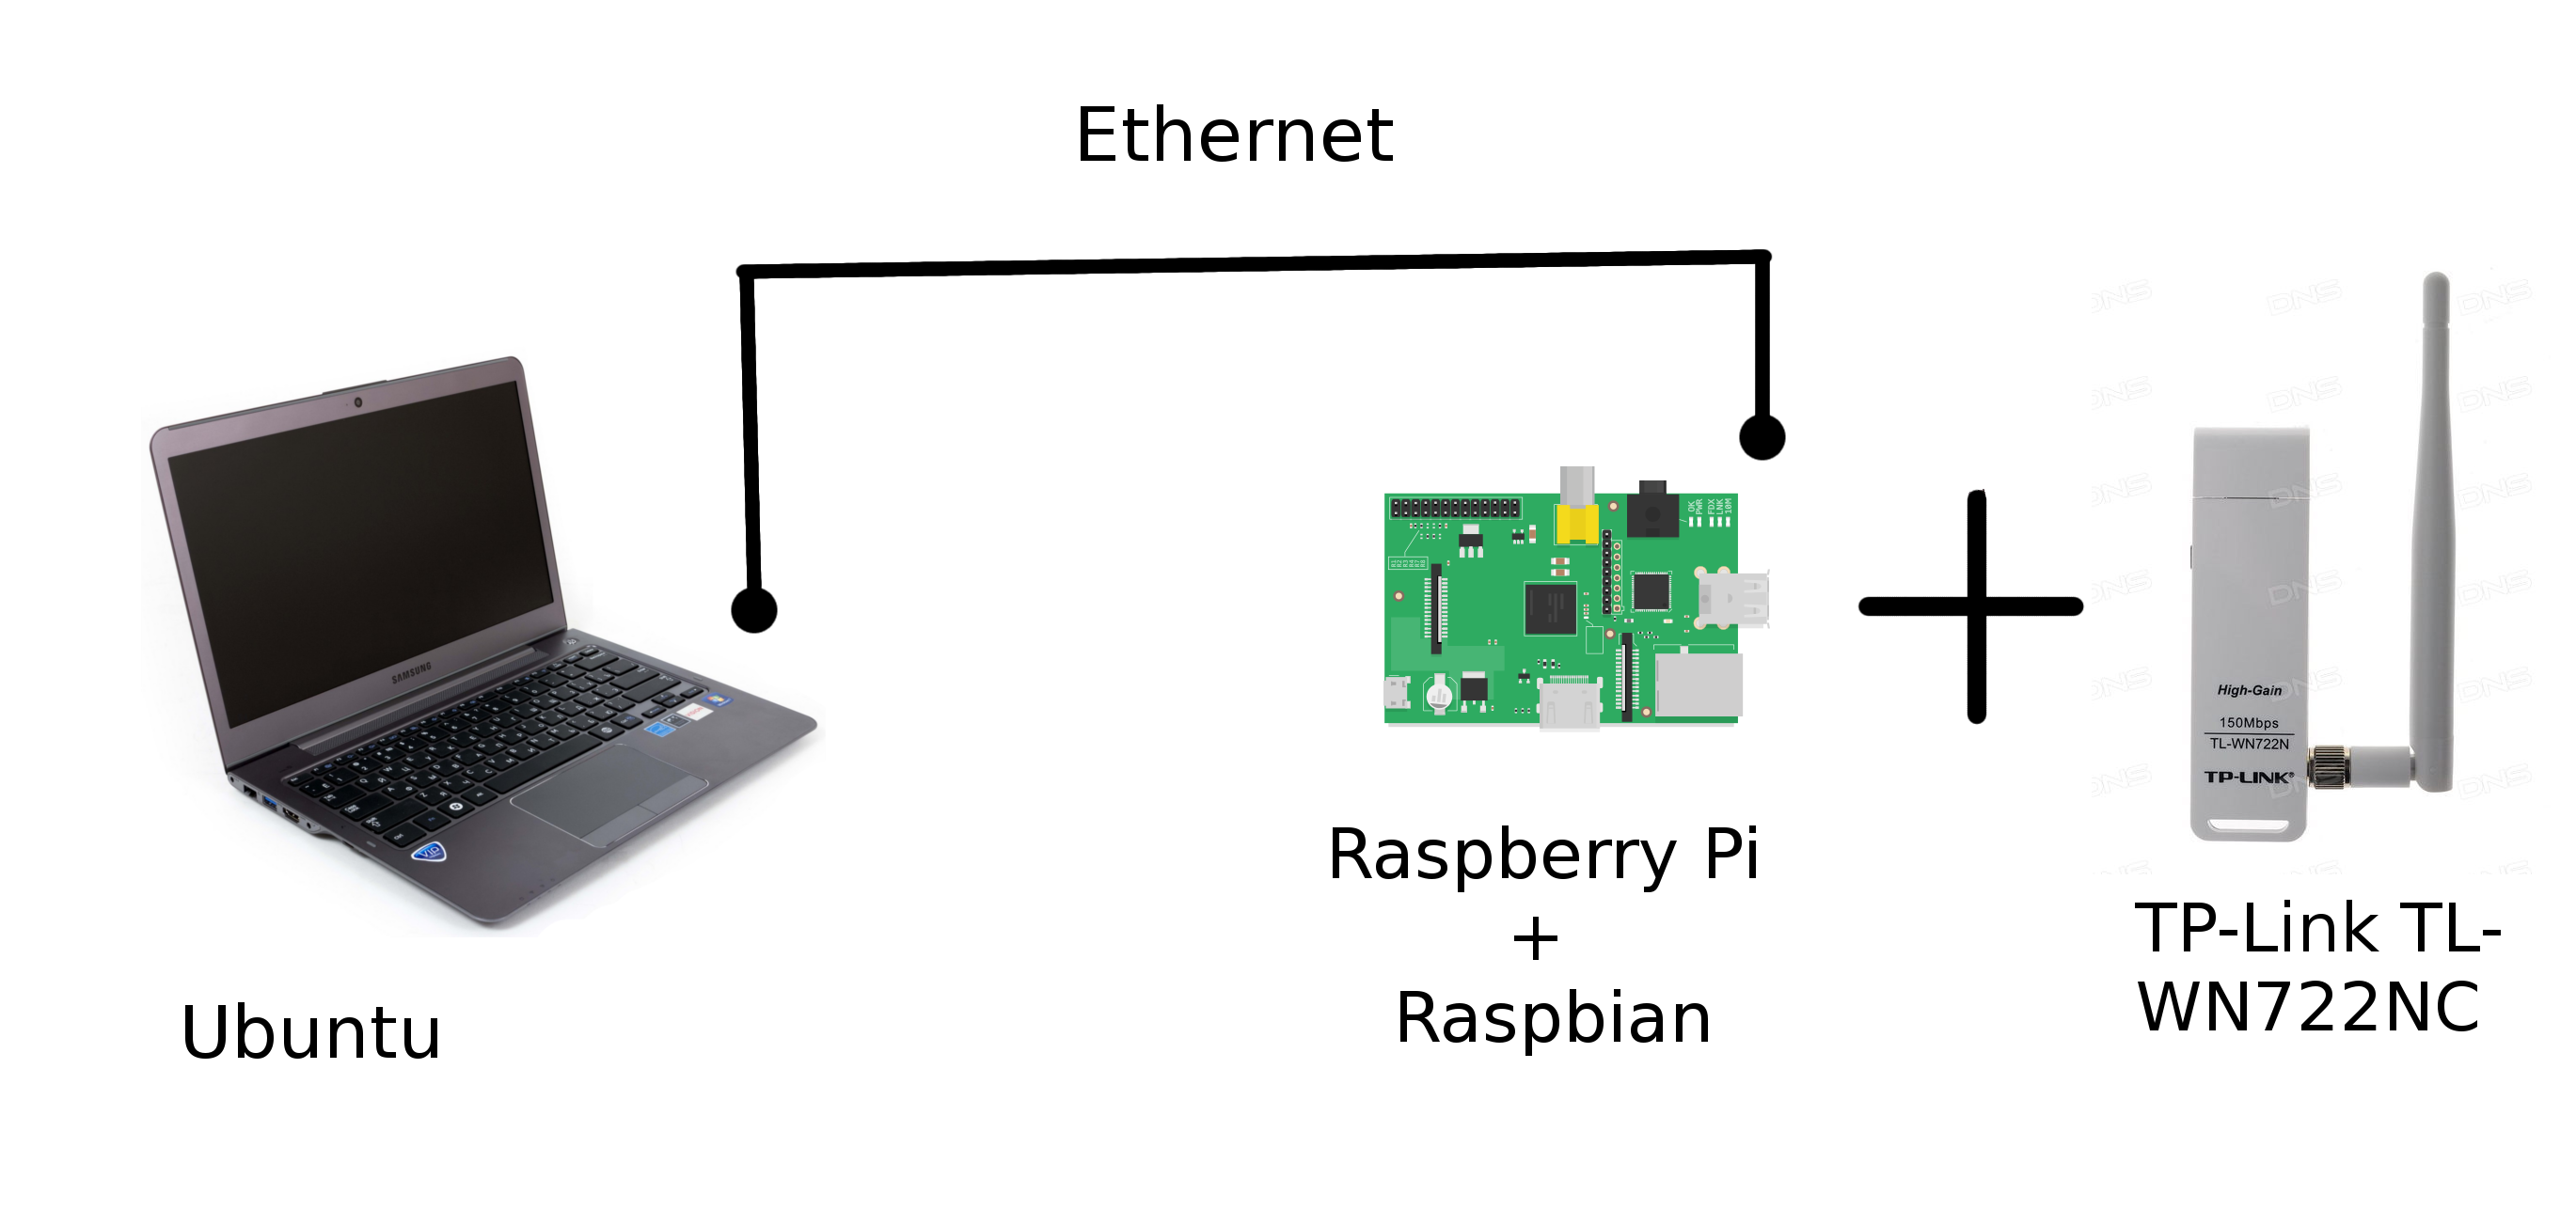
\includegraphics[width=0.9\linewidth]{1}}
\caption{ Схема системы перехвата трафика }
\label{1:1}
\end{figure}

